\documentclass[12pt,a4paper]{report}

% Packages that we are going to use
\usepackage[utf8]{inputenc}
\usepackage[T1]{fontenc}
\usepackage{combelow}% provides \cb to place comma below character
\usepackage[romanian]{babel}
\usepackage{graphicx}
\usepackage{subfiles}
\usepackage{blindtext}
\usepackage[export]{adjustbox} 
\usepackage{geometry}
\usepackage[nottoc,notlot,notlof]{tocbibind}
\usepackage{indentfirst}
\usepackage{amsthm}
\usepackage{listings}
\usepackage{float}
\usepackage[toc,page]{appendix}
\usepackage{subcaption}
\usepackage{makeidx}
\usepackage{geometry}
\usepackage[verbose]{newunicodechar}
\usepackage{hyperref}
\usepackage{amsmath} 
\usepackage[utf8]{inputenc}
\usepackage{chngcntr}
\usepackage{mathtools}
\usepackage[section]{placeins}
\graphicspath{ {figures/} }
\usepackage{array}
\usepackage{afterpage}

\geometry{
	a4paper,
	total={170mm,257mm},
	left=25mm,
	top=25mm,
	bottom=25mm,
	right=25mm,
}

% Line spacing
\renewcommand{\baselinestretch}{1.5} 
\renewcommand\appendixtocname{Anexe}
\renewcommand\appendixname{Anexe}
\renewcommand\appendixpagename{Anexe}
\newcommand\blankpage{%
	\null
	\thispagestyle{empty}%
	\addtocounter{page}{-1}%
	\newpage}

\DeclarePairedDelimiter\norm{\lVert}{\rVert}%
\DeclarePairedDelimiter\abs{\lvert}{\rvert}%

\graphicspath{{images/}{../images/}{figures/}{../figures/}}

\newunicodechar{ș}{\c{s}}
\newunicodechar{Ș}{\c{S}}
\newunicodechar{ț}{\c{t}}
\newunicodechar{Ț}{\c{T}}

\newtheorem{remark}{Observație}[chapter]
\newtheorem{definition}{Definiție}[chapter]
\newtheorem{lemma}{Lemă}[chapter]
\newtheorem{theorem}{Teoremă}[chapter]

\makeindex

\begin{document}

\subfile{chapters/0_first_page}
\restoregeometry

\tableofcontents

\listoffigures

\listoftables

\newpage\null\newpage
\subfile{chapters/01_abstract}

\newpage\null\newpage
\chapter{Introducere}
\section{Motivație}

Anual se produc peste 8 000 de accidente rutiere grave în România, din care rezultă peste 7 000 de răniți grav și peste 2 000 de persoane decedate. Principalul motiv al tuturor acestor incidente, este de departe reprezentat de erorile umane, de la neatenție sau lipsa de experiență până la oboseală.
\begin{figure}[!h]
	\centering
	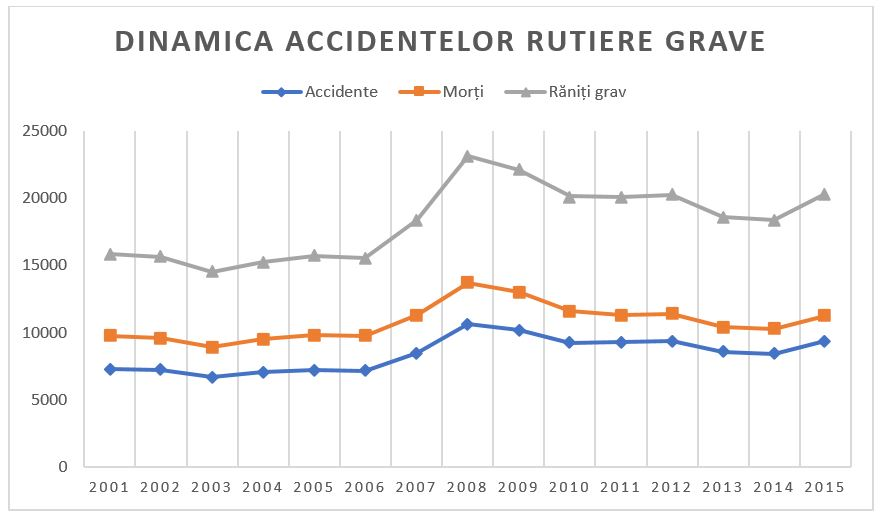
\includegraphics[max width=15cm,max height=15cm,keepaspectratio]{img_1_1}
	\caption[Dinamica accidente rutiere]{Dinamica accidentelor grave produse în România în perioada 2001 - 2015. Statistică preluată din \hyperlink{Dinamicaaccidentelorrutiere}{[8]}.}
\end{figure} 

Însă, o foarte mare parte a erorilor ce cauzează producerea de accidente rutiere pot fi evitate cu ajutorul sistemelor dotate cu inteligență artificială. Sisteme ce pot fi de la cele mai elementare lucruri, precum recunoașterea benzii de circulație până la un sistem complet care poate anticipa și preveni anumite evenimente iminente pe care o persoană le-ar sesiza și evita mult mai încet din punct de vedere al timpului de reacție.

Conform raportului The Atlantic, accidentele rutiere ar putea fi reduse cu până la $90\%$ în jurul anului 2050 datorită sistemelor de asistență cu care sunt actualele mașini dotate dar și sistemele ce vor fi în dotarea viitoarele generații de mașini. \hyperlink{TheAtlantic}{[17]}

Abordarea unei teme de actualitate cu implicații majore în prezent și probabil mult mai intense în viitor, abordarea unei teme ce își propune să vină în ajutorul umanității din prisma faptului că poate scădea semnificativ rata accidentelor rutiere produse ca urmare a greșelilor menționate mai sus, au reprezentat principalele motive ale abordării acestei teme.

\section{Obiective propuse}

Prezenta lucrare de licență are drept obiective prinicpale detecția benzii curente de circulație pe care se află autovehicolul, iar pe baza acestei detecții, cautarea eventualului autovehicol ce se află pe această bandă. 
Acestor două obiective principale li se alătură alte două obiective secundare și anume determinarea distanței față de eventualul autovehicol aflată pe banda detectată și determinarea vitezi relative de deplasare a autovehicolului curente raportat la autovehicolul detectată ca fiind în fața acestuia pe banda de circulație aferentă.

\section{Actualitate}

În ceea ce privește acutalele sisteme de asistență în trafic, cele dezvoltate de Tesla și Waymo (Google) se numără printre cele mai complexe și complete.

\subsubsection{Tesla Autopilot}

Sistemul oferit de Tesla vine în dotare cu 8 camere ce oferă o vizibilitate de 360 de grade până la o distanță de 250 de metri. La acestea se adugă alți 12 senzori ultrasonici cu rolul de a completa vizibilitatea oferită de cele 8 camere. Sistemul dispune și de alți senzori cu rolul de a oferi în plus informații esențiale în detectarea obiectelor. Un radar aplasat în partea frontală a mașinii oferă și mai multe informații fiind capabil să vădă prin ploi ambudente, ceață, praf, chiar și prin mașina din față. \hyperlink{TeslaAutopilotSystem}{[16]}

\begin{figure}[!h]
	\centering
	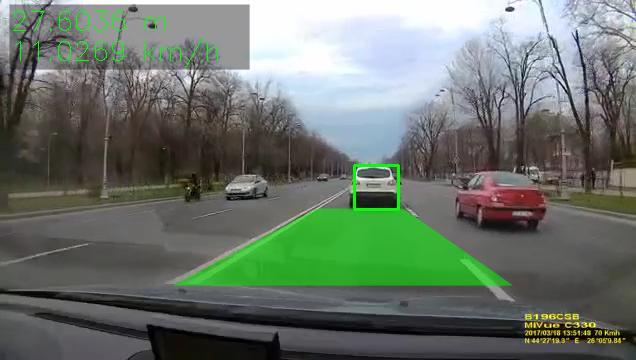
\includegraphics[max width=12cm,max height=12cm,keepaspectratio]{img_1_2}
	\caption[Acoperire sistem Tesla Autopilot]{Acoperire sistem Tesla Autopilot. Imagine preluată din \hyperlink{TeslaAutopilotSystem}{[16]}.}
\end{figure} 

\subsubsection{Waymo}

Autovehicolele Waymo sunt dotate cu senzori și sisteme capabile să detecteze zonele pietonale, bicicliști, alte autovehicole și multe altele pe distanțe similare cu a două terenuri de fotbal. \hyperlink{WaymoSystem}{[20]}

\begin{figure}[!h]
	\centering
	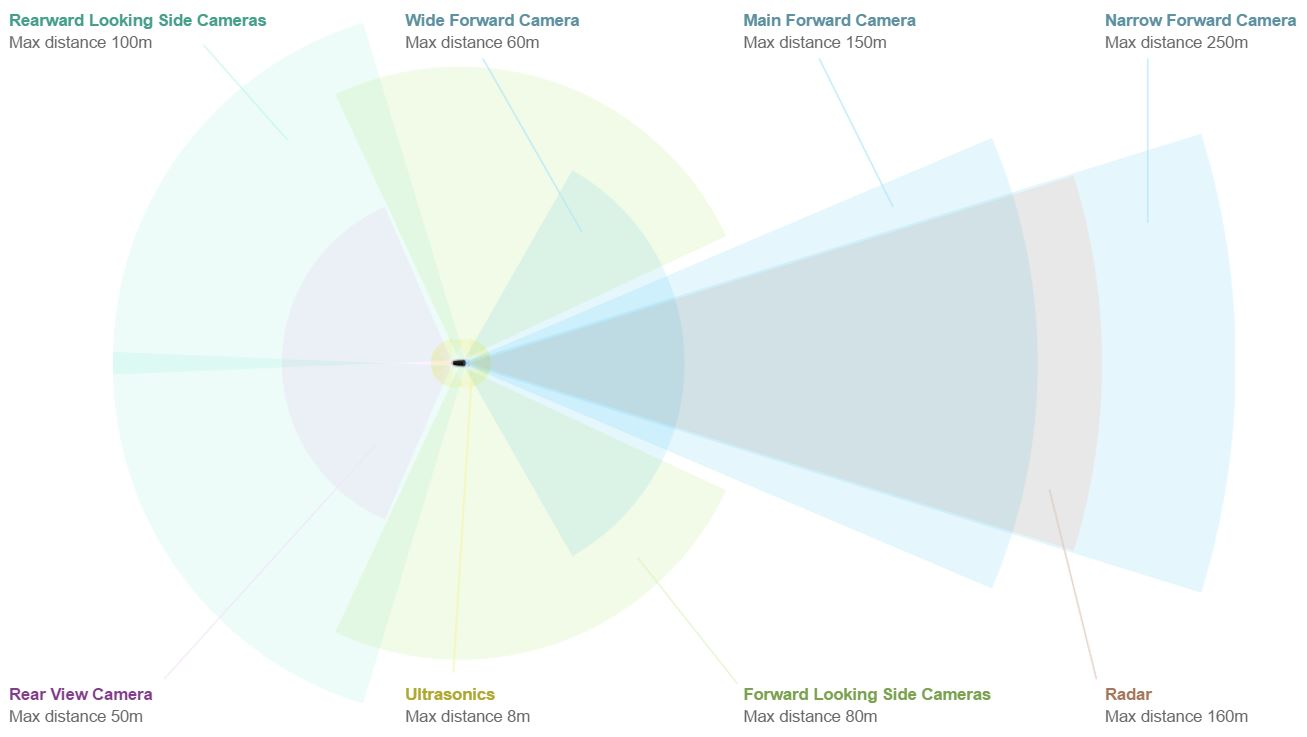
\includegraphics[max width=12cm,max height=12cm,keepaspectratio]{img_1_3}
	\caption[Sistem Waymo]{Sistem Waymo. Imagine preluată din \hyperlink{WaymoSystem}{[20]}.}
\end{figure} 

\section{Structura lucrării}

Prezentarea aplicației realizate debutează prin detalierea fundamentelor teoretice în capitolului II. Aici sunt menționate fundamentele teoretice ce stau la baza realizării acestei prezentei lucrări. 
Capitolul se deschide prin prezentarea noțiunilor despre mașini cu vector suport, un element esențial în antrenarea detectorului de mașini. Pe parcursul acestui capitol prezentăm noțiunile generale despre mașinile cu vector suport, noțiuni despre mașinile cu vector suport multiclasă dar și despre mașinile cu vector suport pentru regresie.

Continuăm prin a descrie histogramele de gradienți orientați folosite în extragerea de caracteristici din imagini. Aceste caracteristici sunt trimise mașinilor cu vectori suport pentru antrenarea dar sunt folosite ulterior și pentru testarea și validarea potențialelor zone ce conțin mașini. 
Se prezintă pe lângă noțiunile generale și etapele algoritmului de extragere a caracteristicilor prin această metodă. 

Metoda glisării ferestrei este și ea abordată în fundamentarea teoretică, această metodă este cea care sta la baza identificării zonelor din imagine pentru care detectorul produce scoruri pozitive în ceea ce privește detecția de autovehicole.

În finalul acestui capitol este prezentată noțiunea de IPM, noțiune esențială în detectarea benzii de circulație, pe de o parte, dar și în analiza datelor privind distanța față de autovehicolul aflăt pe banda curentă și de viteza relativă a acestuia în maniera abordată de lucrare de față.

Capitolul III este dedicat procesului propriu-zis de dezvoltare al aplicației. Începe prin prezentarea componentei ce se ocupă de detectarea benzi. Continuăm prin prezentarea componentei care determină pozițiile eventualelor autovehicole din imagini și vom incheia prin prezentarea metodelor abordate de detectare a distanței față de autovehicolul din față pe banda curentă de circulație împreună cu viteza relativă în raport cu ea.

Spre finalul lucrării, în capitolul IV, vor fi prezentate bazele de date utilizate atât în cadrul componentei ce se ocupă de detectarea benzii de circulație cât și a componentei ce se ocupă de detectarea de autovehicole. Pentru fiecare dintre acestea vor fi prezentate informații generale despre respectiva bază de date, tipurile de imagini pe care le conține, algoritmii de evaluare utilizați pentru validarea rezultatelor obținute, dar și rezultatele propriu-zise.

În închierea lucrării vor fi trase concluziile finale și vor fi prezentate posibile viitoare direcții de dezvoltare ale curentei aplicații.

\newpage\null\newpage
\chapter{Fundamente teoretice}
\section{Mașini cu vector suport}

\subsection{Noțiuni generale}

Mașinile cu vector suport au devenit populare în ultimii ani pentru rezolvarea problemelor de clasificare sau regresie. Acestea realizează o clasificare de tip două clase prin folosirea modelului liniar de forma
\begin{align}
	y(x) = w^T\phi(x) + b
\end{align}
unde $\phi$ este o transformare a spațiului caracteristic.

Datele de antrenare sunt alcătuite din N vectori de intrare $x_1, ...,x_N$ fiecare dintre aceștia având asociate valorile $t_1, ...,t_N$ din mulțimea $t_n \in \{-1,1\}$, iar rezultatul din $y(x)$ reprezintă scorul asociat vectorului de intrare $x$.

De asemenea trebuie să ne asigură că în momentul antrenării setul de date este liniar separabil în spațiul caracteristicilor ceea ce înseamnă că pentru orice alegere a parametrilor $w$ și $b$ dacă funcția $y(x_n) > 0$ atunci valoarea asociată trebuie să fie $t_n = +1$. Situația este similară și pentru cazul în care $y(x_n ) < 0$, atunci valoarea asociată trebuie să fie $t_n = -1$. 
Concluzionând cele două proprietăți menționate anterior putem afirma faptul că următoarea inecuație trebuie să fie mereu validă  $t_n y(x_n) > 0$. 

Mașinile cu vector suport abordează problema prin conceptul de „margine” ce este definită ca fiind cea mai mică distanță dintre o frontieră de decizie și orice exemplu primit. O ilustrație a acestui fapt se poate vedea în figura 2.1.
\begin{figure}[!h]
	\centering
	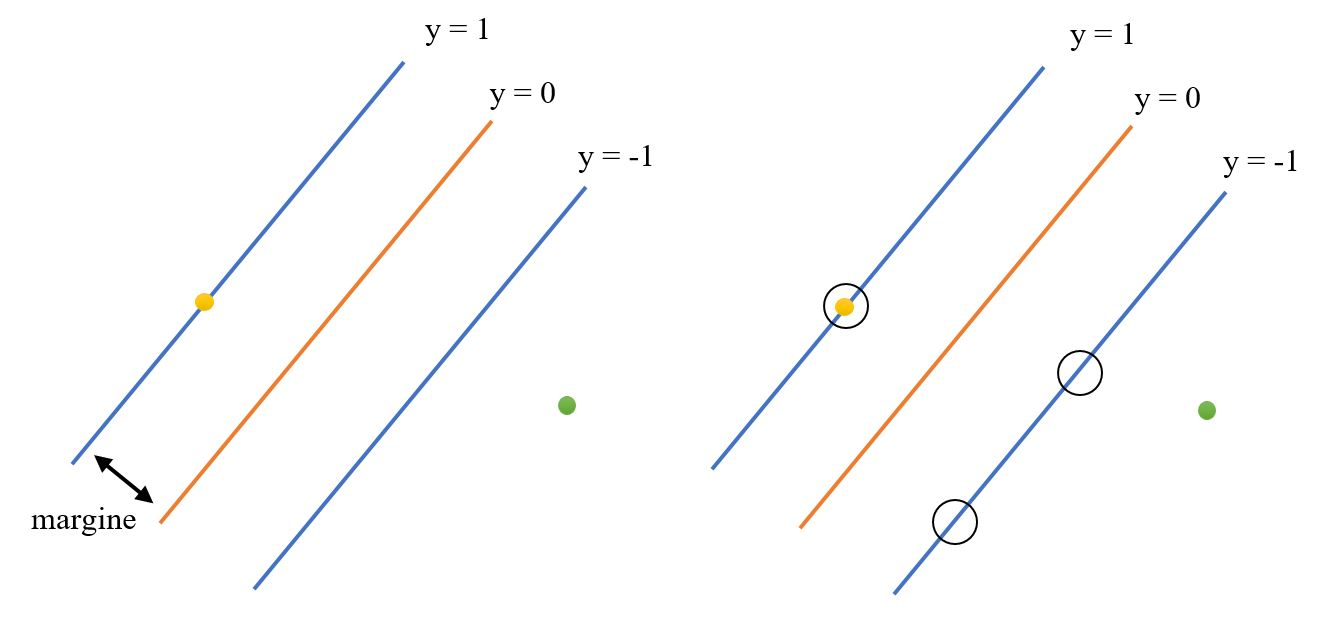
\includegraphics[max width=10cm,max height=10cm,keepaspectratio]{img_2_1}
	\caption[Mașini cu vector suport]{Marginea este definită ca distanța perpendiculara dintre limita de decizie și cel mai apropiat punct, după cum se poate observa în figura din stânga. Maximizăm limita marginii precum în figura din dreapta. Locația acestei limite este determinată de mașinile cu vectori suport indicate prin cercuri.}
\end{figure} 

În cazul mașinilor cu vectori suport, limita de decizie este aleasă să fie drept locația unde „marginea” este maximă. Această decizie este motivată de folosirea „teoriei computaționale de învățare” cunoscută drept „teoria statistică de învățare”. 

Primul model de distribuție peste vectorii de intrare $x$ pentru orice clasa folosește densitatea Parzen cu un nucleu Gaussian având parametrul comun $\sigma^2$. Utilizarea limitei optime determină cel mai bun hiperplan prin minimizarea probabilității de eroare relative densității modelului învățat. 

În cazul limitei $\sigma^2 \rightarrow 0$, hiperplanul optim este cel care are marginea maximă. Intuitiv, deoarece $\sigma^2$ este redus, hiperplanul este dominat mai mult de punctele din apropiere decât de cele din depărtare, în limită hiperplanul devenind independent de datele ce nu sunt mașini cu vector suport \hyperlink{ChristopherBishop}{[8]}. 

\subsection{Mașini cu vector suport multiclasă}

În principiu, mașinile cu vector suport sunt clasificatori de tip două clase însă, în practică întâlnim multe cazuri în care avem nevoie de probleme ce presupun mai mult de două clase. De-a lungul timpului au fost propuse diferite variante de rezolvare a problemei construcției mașini cu vector suport multiclasă.

Cea mai cunoscută abordarea (Vapnik, 1998) este reprezentată de construcția a K mașini cu vectori suport separate, unde în fiecare $k^{th}$  model, $y_k(x)$ este antrenat folosind date din clasa $C_k$ pe post de date de antrenare pozitive, iar datele din celelalte $K-1$ clase rămase pe post de date de antrenare negative. Această tehnică este cunoscută sub numele de „unul-versus-toți”. 

Astfel noile predicții pentru un input $x$ for fi făcute pe baza următoarei relații
\begin{align}
	y(x) = \max_{\substack{k}}y_k(x)
\end{align}

Evident, în această abordare pot apărea anumite probleme precum cea legată de faptul că acești clasificatori au fost antrenați pe diferite clase, ceea ce înseamnă că nu avem neapărat o garanție a faptului că se vor comporta în practică pe tipuri diferite de intrări similar cu datele de antrenare.

O altă problemă întâlnită în această abordare de unu-versus-toți este legată de cantitatea datelor de antrenare în sensul de pierdere al echilibrului dintre exemplele pozitive și cele negative. Spre exemplu, să presupunem că avem 10 tipuri de clase. Pentru o instanță a unei mașini cu vector suport vom avea $10\%$ dintre toate datele de antrenare disponibile încadrate precum exemple pozitive, iar cealaltă parte, mult mai densă, de $90\%$ vor reprezenta exemple de antrenare negative, fapt ce va crea o discrepanță foarte mare între ele, astfel simetria fiind pierdută.

Weston and Watkins (1999) definesc o singură funcție obiectiv pentru antrenarea tuturor celor $K$ vectori suport mașină simultan, acest procedeu fiind bazat pe maximizarea marginilor pentru fiecare clasă. Acest lucru produce un efect de rulare înceată a antrenării deoarece rezolvarea a $K$ probleme separate de optimizare ar însemna că pentru fiecare $N$ punct de date are un cost de rulare per total de $O(KN^2)$, iar o singură problemă de optimizare cu dimensiunea $(K - 1)N$ poate fi rezolvată cu un cost total de $O(K^2N^2)$.

Una dintre cele mai întâlnite metode de rezolvare a acestor probleme este o abordare în care vom antrena $K(K-1)/2$ vectori suport mașină diferiți pentru toate perechile de clase posibile, iar rezultatul final va fi determinat de aceea mașină cu vector suport care va răspunde cu un număr cât mai mare de voturi (scor) dintre toate cele $K(K-1)/2$ posibilități. Această este numită deseori drept o antrenare „unu-versus-unu”. Evident, în această situație timpul de rulare va crește odată cu numărul claselor pentru care trebuie antrenate mașinile cu vector suport.

Pentru a rezolva această problemă a timpului de execuție putem organiza perechile de clasificare într-un graf aciclic. Astfel, pentru K clase pe care le avem de analizat vom avea în total $K(K-1)/2$ vectori suport mașină, iar pentru a clasifica o intrare vom avea nevoie doar de $K-1$ perechi de clasificatori spre a fi evaluați cu clasificatorii specifici traversări grafului.

O abordare diferită a clasificării multiclasă în cazul mașinilor cu vectori suport, bazată pe coduri de ieșire corectoare de erori dezvoltate de Dietterich și Bakiri (1995) și ulterior aplicate pe mașini cu vector suport de către Allwein, Schapire și Singer (2000). 
Acest lucru poate fi văzut precum o generalizare a schemei de vot unu-versus-unu în care cele mai generale părți ale clasei sunt folosite pentru formarea de clasificatori individuali.
Cele $K$ clase sunt representate precum seturi particulare de răspunsuri provenite din clasificatori de două clase, iar împreună cu o schemă de decodare potrivită oferă robustețe la erori și la ambiguitatea rezultatelor clasificatorilor individuali.

Deși clasificarea cu mașini vectori suport multiclasă încă are multe capitole de îmbunătățit, în practică abordarea unul-versus-toți rămâne cea mai utiliza în ciuda limitărilor de performanță aferente \hyperlink{ErinAllweinRobertSchapireYoramSinger}{[9}, \hyperlink{JasonWestonSimonWatkins}{10}, \hyperlink{ThomasDietterichGhulumBakiri}{18}, \hyperlink{VladimirVapnik}{19]}.

\subsection{Mașini cu vector suport pentru regresie}

În regresia liniară simplă se minimizează o funcție de eroare regularizată definită de
\begin{align}
	\frac{1}{2}\sum_{n=1}^{N}\{y_n-t_n\}^2+\frac{\lambda}{2}\norm w^2
\end{align}

Pentru a obține soluțiile, funcția cuadrică de eroare va fi înlocuită de o funcție numită $\epsilon$ - funcție de eroare intensivă (Vapnik, 1995) ce ne returnează eroarea 0 dacă diferența absolută dintre predicția $y(x)$ și asocierea sa $t$ este mai mică decât $\epsilon$ unde $\epsilon > 0$. Un exemplu simplu de $\epsilon$ - funcție de eroare intensivă cu un cost liniar asociat cu eroarea din exteriorul regiunii este
\begin{align}
	E_{\epsilon}(y(x) - t) = 
	\begin{cases}
	0,& \text{dacă } \abs {y(x) - t} < \epsilon\\
	\abs {y(x) - t} - \epsilon,              & \text{altfel}
	\end{cases}
\end{align}
exemplu ilustrat în figura 2.2.
\begin{figure}[!h]
	\centering
	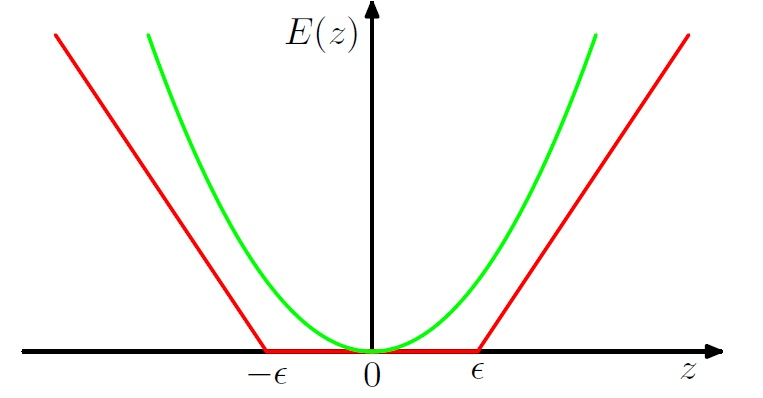
\includegraphics[max width=10cm,max height=10cm,keepaspectratio]{img_2_2}
	\caption[Mașini cu vector suport pentru regresie]{Cu roșu se poate observa $\epsilon - functie de eroare intensivă$, iar cu verde se poate observa o funcție cuadrică de eroare. Imagine preluată din \hyperlink{ChristopherBishop}{[8]}.}
\end{figure}
 
Prin urmare, vom minimiza o funcție de eroare regularizata dată prin
\begin{align}	
	C\sum_{n = 1}^{N}E_{\epsilon}(y(X_n) - t_n) + \frac{1}{2}\norm w ^ 2
\end{align}

Similar cu cele prezentate anterior putem alege un prag $\xi_n \geq 0$ și $ \widehat{\xi_n} \geq 0$, unde $\xi_n > 0$ corespunde punctului pentru care următoare condiție este îndeplinită $t_n > y(x_n) + \epsilon$, iar  $ \widehat{\xi_n} \geq 0$ corespunde punctului pentru care următoarea condiție este îndeplinită $t_n < y(x_n) - \epsilon$. Acestea fiind ilustrate în figura 2.3.
\begin{figure}[!h]
	\centering
	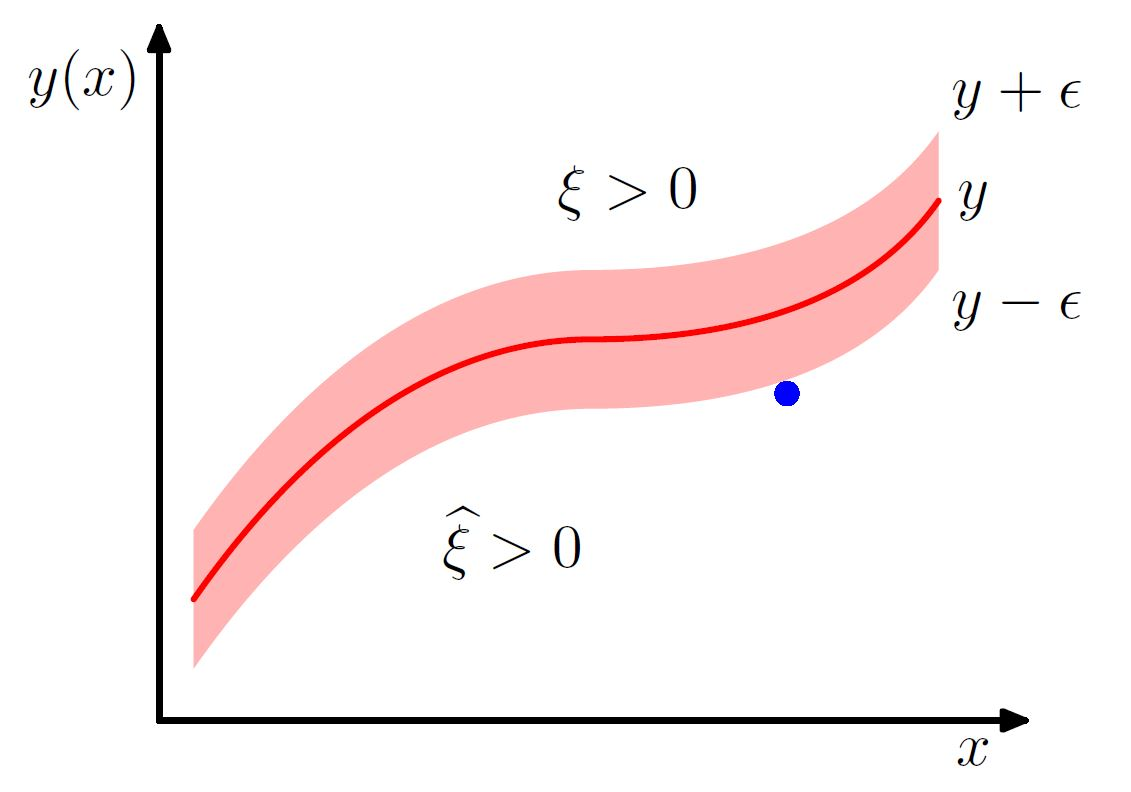
\includegraphics[max width=10cm,max height=10cm,keepaspectratio]{img_2_3}
	\caption[Mașini cu vector suport pentru regresie 2]{Este prezentată o regresie vector suport mașină evidențiind curba de regresie împreună cu zona $\epsilon – intensiv$. De asemenea, sunt prezentate variabilele $\xi$ și $ \widehat{\xi}$. Punctele de deasupra zonei $\epsilon$ au $\xi > 0$ și $ \widehat{\xi} = 0$, iar punctele de sub zona $\epsilon$ au $\xi = 0$ și $ \widehat{\xi} > 0$, în cele din urmă, punctele din interiorul zonei $\epsilon$ au $\xi = 0$ cât și $ \widehat{\xi} = 0$. Imagine preluată din \hyperlink{ChristopherBishop}{[8]}.}
\end{figure}

Condiția ca un punct să fie în interiorul zone $ \epsilon $ este ca $y_n - \epsilon \leq t_n \leq y_n + \epsilon$ unde $y_n = y(x_n)$. Introducând variabilele $\xi_n$ și $\widehat{\xi_n}$ permitem punctelor să se afle în afara zonei de interes condiționat de faptul că variabilele introduse sunt nenule iar următoarele condiții sunt indeplinite
\begin{align}	
	t_n \leq y(x_n) + \epsilon + \xi_n
\end{align}
\begin{align}	
	t_n \geq y(x_n) - \epsilon - \widehat{\xi_n}
\end{align}

În practică, în detrimentul fixării unui parametru $\epsilon$ se preferă fixarea unui parametru $v$ ce are drept rol principal limitarea punctelor din afara zonei $\epsilon$. O rezolvare a unei probleme de regresie având un set de date sinusoidal cu vectori suport mașină este ilustrată în figura 2.4. În această situație parametrii $v$ și $C$ au fost aleși manual, însă în practică aceste valori sunt determinate automat \hyperlink{ChristopherBishop}{[8]}.
\begin{figure}[!h]
	\centering
	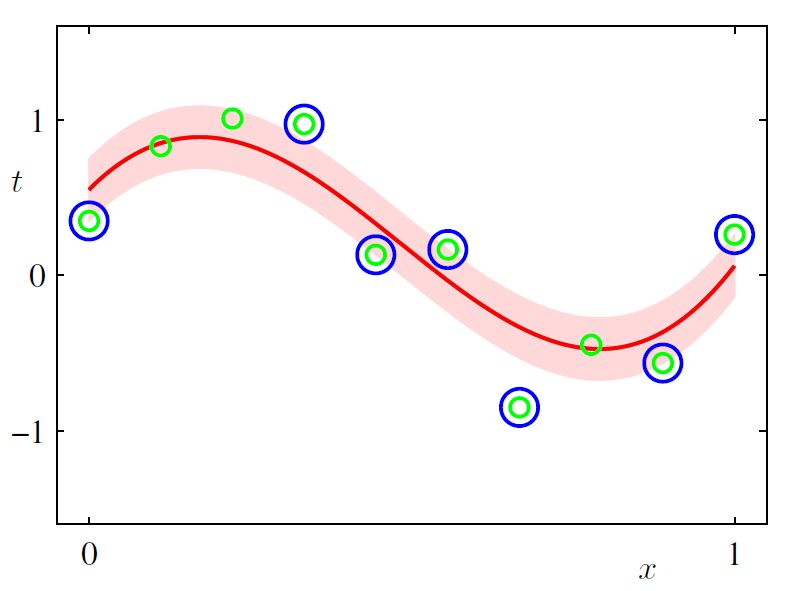
\includegraphics[max width=10cm,max height=10cm,keepaspectratio]{img_2_4}
	\caption[Mașini cu vector suport pentru regresie 3]{Este prezentată un vector suport mașină pentru regresie aplicat pe un set de date sinusoidal și utilizând un nucleu Gaussian. Curba de regresie prezisă este ilustrată prin linia roșie, iar zona $\epsilon - intensiv$ este ilustrată prin zona roșie hașurată. Datele sunt indicate prin cercurile verzi, iar vectorii suport mașină sunt indicați prin cercurile albastre. Imagine preluată din \hyperlink{ChristopherBishop}{[8]}.}
\end{figure}

\section{Histograme de gradienți orientați}

\subsection{Noțiuni generale}

Histograma de gradienți orientați este un descriptor utilizat în vederea artificială și în procesarea imaginilor cu scopul de a detecta obiecte. 

Prin această tehnică se numără aparițiile orientării gradientului în anumite porțiuni localizate ale imaginii.

Ideea principală ce stă la baza histogramei de gradienți orientați este reprezentată de faptul că aspectul și forma obiectului dintr-o imagine pot fi descrise prin distribuirea intensității gradienților sau a muchiilor direcțiilor. În figura 2.5 este prezentat un exemplu practic.
\begin{figure}[!h]
	\centering
	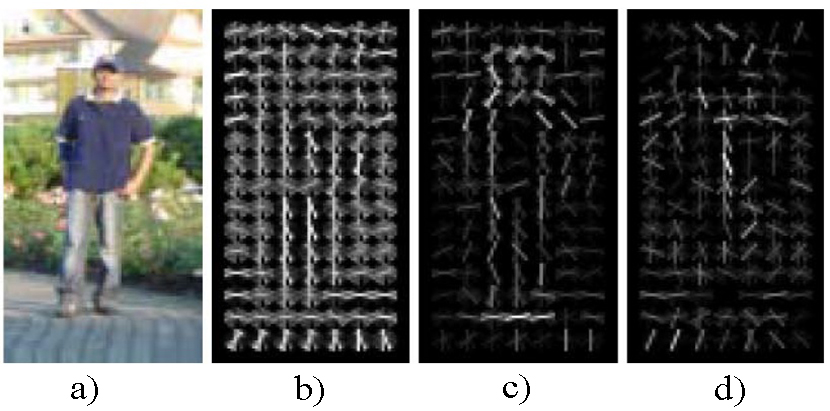
\includegraphics[max width=10cm,max height=10cm,keepaspectratio]{img_2_5}
	\caption[Descriptor HOG]{(a) imaginea originală; (b) descriptorul histogramei de gradienți orientați asociate imaginii; (c) valorile pozitive din $w$ a descriptorul histogramei de gradienți orientați asociate imaginii; (d) valorile negative din $w$ a descriptorul histogramei de gradienți orientați asociate imaginii. Imagine preluată din \hyperlink{NavneetDalalBillTriggs}{[12]}.}
\end{figure}

Imaginea este împărțită în mici regiuni conectate numite celule, iar pentru pixelii din fiecare celulă se obține o histogramă de gradienți orientați. Descriptorul este rezultatul concatenării acestor histograme. Se poate îmbunătății acuratețea prin normalizarea histogramelor, această normalizare are ca rezultat o invarianță mai bună a schimbărilor intensităților luminii sau apariției umbrelor. În figura 2.6 sunt reprezentate vizual aceste noțiuni.
\begin{figure}[!h]
	\centering
	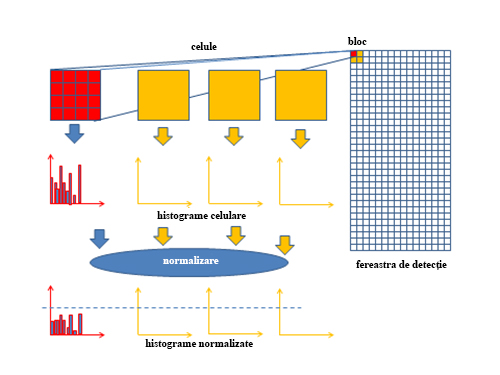
\includegraphics[max width=10cm,max height=10cm,keepaspectratio]{img_2_6}
	\caption{Procesul de extragere a histogramelor de gradienți orientați}
\end{figure}

Histogramele de gradienți orientați prezintă principalul avantaj prin faptul că lucrează la nivel de celulă locală, astfel, în practică, se comportă bine la invarianța geometrică și transformările fotometrice, exceptând, desigur, orientarea obiectului \hyperlink{RichardSzeliski}{[13]}. 

\subsection{Etapele metodei}

\subsubsection {Compunerea gradientului}

Principalul pas în majoritatea determinării de caracteristici în preprocesarea de imagini este de a asigura o normalizarea a valorilor aspura culorii. Astfel, primul pas constă în determinarea valorii gradienților, iar cea mai comună metodă pentru a face acest lucru este să aplicăm un filtru $1-D$ centrat, atât pe direcția verticală cât și pe direcția orizontală. Pentru acest lucru se pot utiliza următoarele nuclee de filtre
\begin{align}	
	[-1, 0, 1]  \quad sau  \quad  [-1, 0, 1]^T
\end{align}

\subsubsection {Orientarea binară}

În continuare trebuie create histogramele de celule. Fiecare pixel dintr-o celulă primește un vot ponderat pentru o poziție pe un canal orientat al histogramei. Canalele histogramei sunt distribuite uniform intre 0 și 180 de grade sau intre 0 și 360 de grade. În practică, pentru a determina contribuția pixelilor se folosește magnitudinea gradientului.

\subsubsection {Blocurile descriptor}

Datorită diferitelor situații în care iluminarea și contrastul pot varia, este nevoie de normalizarea locală a gradientului, ceea ce presupune gruparea celulelor în blocuri mai mari, iar ulterior concatenarea mai multor blocuri formează descriptorul histogramei de gradienți orientați.

\subsubsection {Normalizarea blocului}

În ceea ce privește normalizarea blocurilor putem folosi mai multe metode propuse de Dalal și Triggs. În continuare vom presupune că $v$ este vectorul ce nu este normalizat și ce conține histogramele, $\norm{v}_k$ reprezintă norma vectorului, pentru $k = 1,2$ la care adugăm și o constantă $e$. Din acestea deducem următoarele forme de normalizare
\begin{align}	
	L2-norm: f = \frac{v}{\sqrt{\norm{v}_2^2 + e^2}}
\end{align}
\begin{align}	
	L1-norm: f = \frac{v}{\norm{v}_1 + e}
\end{align}
\begin{align}	
	L1-sqrt: f = \sqrt{\frac{v}{\norm{v}_1 + e}}
\end{align}
Toate aceste metode de normalizare oferă o îmbunătățire semnificativă făță de datele nenormalizate, iar cea care pare a se comporta puțin mai bine în detrimentul celorlalte este $L1-norm$.

\subsubsection {Clasificarea cu suport vector mașină}

Pasul final în procesul de detecție folosind histogramele de gradienți orientați este de a antrena clasificatori cu descriptorii obținuți. Clasificarea cu vectori suport mașină poate fi o variantă.

\subsubsection {Clasificarea cu rețele neuronale}

În cazul în care se dorește o acuratețe de clasificare mai bună se pot folosi rețele neuronale în detrimentul vectorilor suport mașină \hyperlink{NavneetDalalBillTriggs}{[12]}.

\section{Metoda glisării ferestrei}

\subsection{Noțiuni generale}

Tehnica de glisare a ferestrei este una des întâlnită în detectarea de obiecte în imagini. Aceasta presupune deplasarea ferestrei pe toată suprafața imaginii cu un anumit salt de pixel stabilit în prealabil. De asemenea, această tehnică poate fi folosită pentru diferite dimensiuni de detecție. Astfel avem ca alternative, fie să mărim sau să micșorăm dimensiunea ferestrei glisante, fie să mărim sau să micșorăm dimensiunea imaginii și să rulăm aceeași dimensiune a ferestrei pe diferite dimensiuni ale imaginii \hyperlink{RichardSzeliski}{[13]}.

Tehnica prezentată anterior este ilustrată și în figura 2.7 sau în figura 2.8
\begin{figure}[!h]
	\centering
	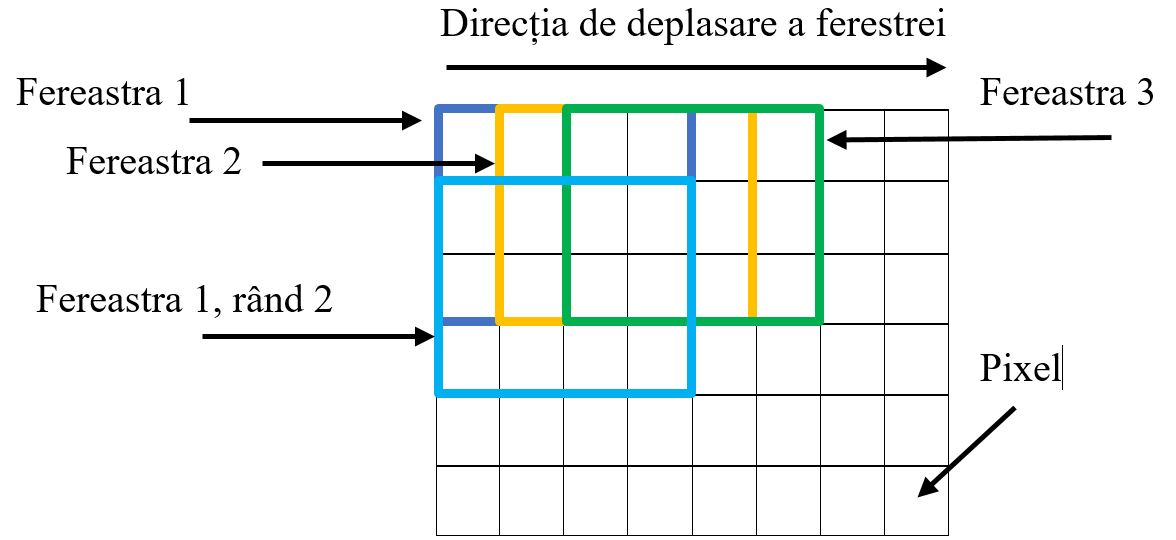
\includegraphics[max width=10cm,max height=10cm,keepaspectratio]{img_2_7}
	\caption{Metoda glisării ferestrei la nivel de concept}
	\label{fig:nonfloat}
\end{figure}
\begin{figure}[!h]
	\centering
	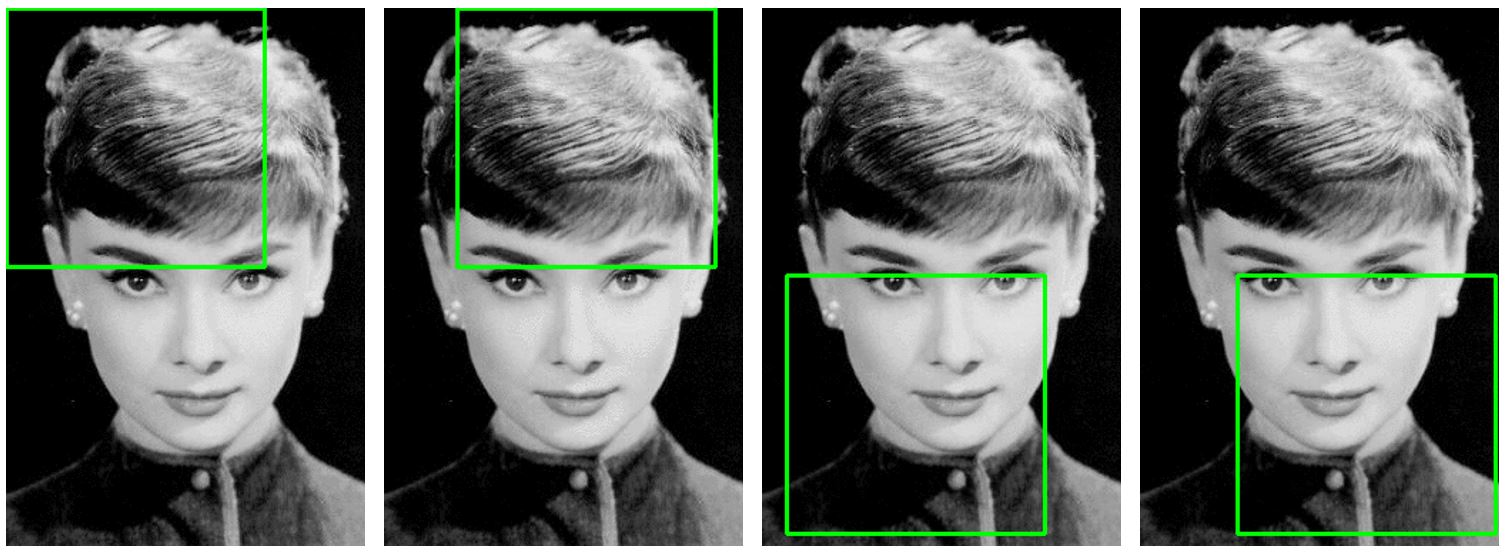
\includegraphics[max width=15cm,max height=15cm,keepaspectratio]{img_2_8}
	\caption{Metoda glisării ferestrei în practică, în patru momente diferite}
	\label{fig:nonfloat}
\end{figure}

\section{IPM (Inverse Perspective Mapping)}

\subsection{Noțiuni generale}

IPM-ul reprezintă o tehnică de transformare geometrică care proiectează fiecare pixel a unui obiect din 3D într-o perspectivă 2D. Acest lucru înseamnă repoziționarea fiecărui pixel într-o poziție nouă corespunzătoare noii perspective, astfel construindu-se noua imagine. Din punct de vedere matematic acest lucru poate fi descris printr-o proiecție din planul Euclidian 3D de forma $W = \{(x,y,z)\} \in E^3$ într-un plan 2D de forma $I = \{(u,v)\} \in E^2$. Această transformare mai poartă numele și de „Bird's eye view” datorită privirii de sus pe care o oferă asupra imaginii originale. În figura 2.9 este prezentat vizual acest model.

\begin{figure}[!h]
	\centering
	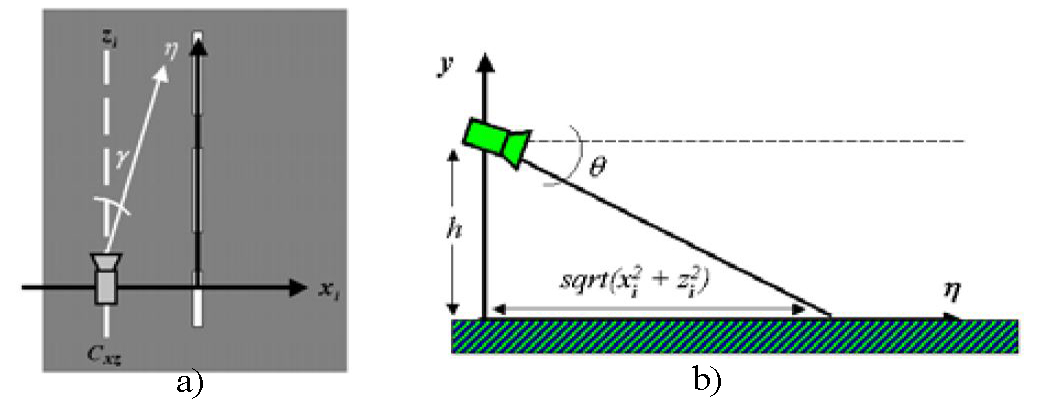
\includegraphics[max width=15cm,max height=15cm,keepaspectratio]{img_2_9}
	\caption[Modelul IPM]{a) vizualizarea geometrică „de sus” în planul construit; b) vizualizarea geometrică din lumea reală. Imagine preluată din \hyperlink{AnuarMikdadMuadAiniHussainSalinaAbdulSamadMohdMarzukiMustaffaBurhanuddinYeopMajlis}{[1]}.}
	\label{fig:nonfloat}
\end{figure}

Pentru aflarea coordonatelor în noul plan putem folosi următoarele formule 2.12 și 2.13 rezultate pe baza modelului IPM.

\begin{align}	
	u(x,0,z) = \frac{\gamma(x,0,z) - (Y-\alpha)}{\frac{2\alpha}{n-1}}
\end{align}
\begin{align}	
	v(x,0,z) = \frac{\theta(x,0,z) - (\Theta - \alpha)}{\frac{2\alpha}{m-1}}
\end{align}

În formulele prezentate au fost folosite:

$\gamma = tan^{-1}(\frac{z}{x})$;

$\theta = tan^{-1}(\frac{h}{\sqrt{x^2+z^2}})$;

$Y$ - reprezintă unghiul dintre proiecția axei optice pe planul real; 

$\Theta$ - reprezintă unghiul dintre proiecția axei optice și planul orizontal;
 
$\alpha$ - reprezintă unghiul de înclinație al camerei;

$m \times n$ reprezintă rezoluția imaginii.

În figura 2.10 se poate observa un exemplu practic al IPM-ului.

\begin{figure}[!h]
	\centering
	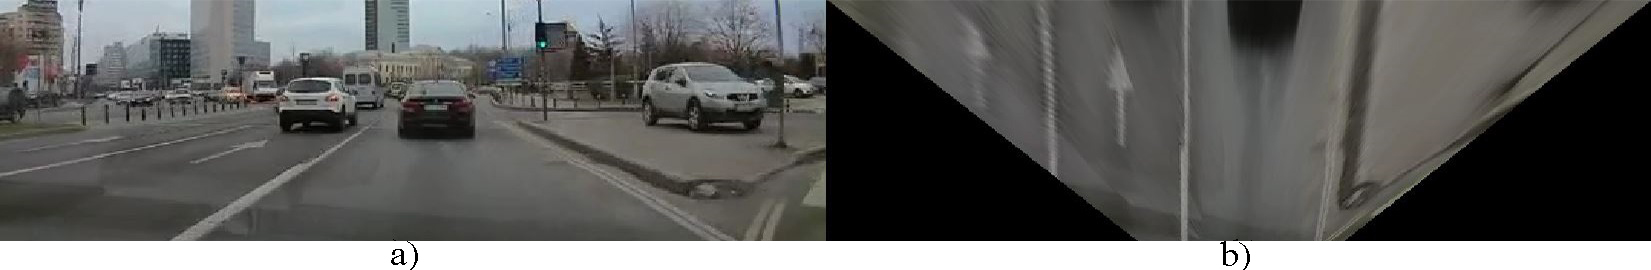
\includegraphics[max width=17cm,max height=17cm,keepaspectratio]{img_2_10}
	\caption[Imagine IPM]{Imaginea IPM (b) asociată unei imaginii din plan real (a).}
	\label{fig:nonfloat}
\end{figure}

Evident, formulele prezentate anterior prezintă un dezavantaj datorită faptului că procesarea prin intermediul lor se face pixel cu pixel. În elaborarea lucrării practice au fost folosite metode de obținere a IPM-ului mult mai rapide pentru a îndeplini unul dintre obiectivului lucrării și anume rularea în timp real a aplicației.

\begin{figure}[!h]
	\centering
	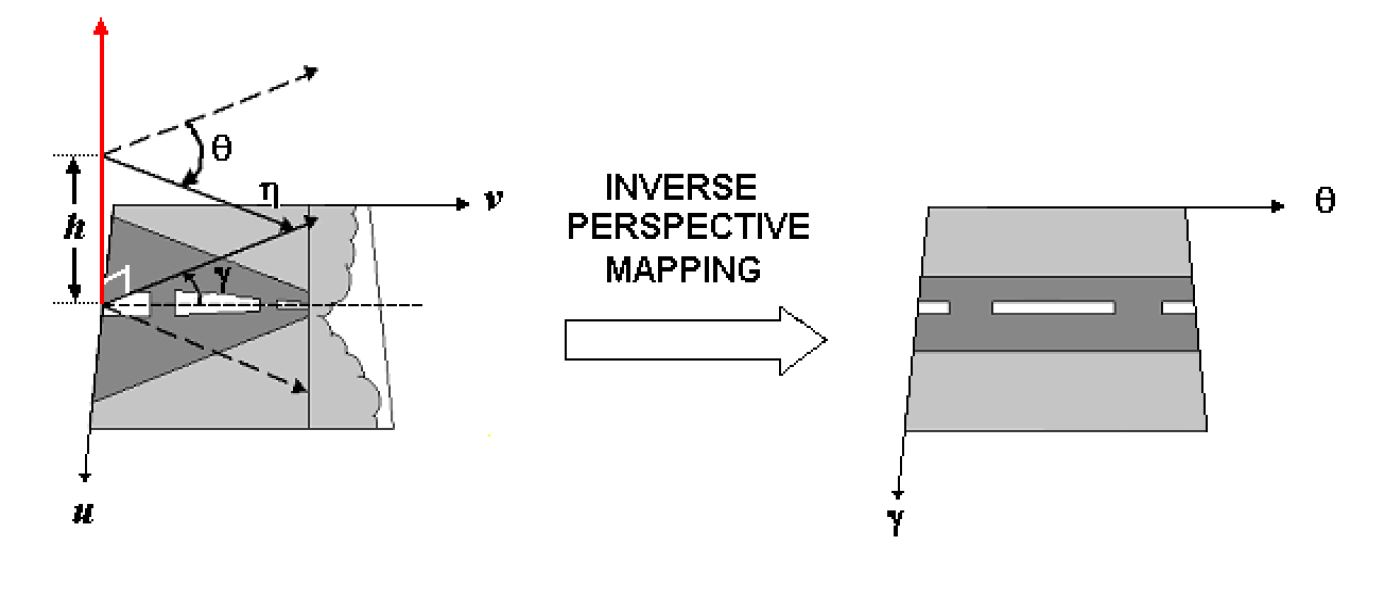
\includegraphics[max width=17cm,max height=17cm,keepaspectratio]{img_2_11}
	\caption[Reprezentare grafică IPM]{Reprezentarea grafică a IPM. Imagine preluată din \hyperlink{AnuarMikdadMuadAiniHussainSalinaAbdulSamadMohdMarzukiMustaffaBurhanuddinYeopMajlis}{[1]}.}
	\label{fig:nonfloat}
\end{figure}

\chapter{Dezvoltarea aplicației}
\section{Detectare bandă}
\subsection{Noțiuni introductive}
O primă componentă a aplicației de față este ceea care se ocupă de detecția benzi curente de circulație. Scopul acesteia este de a identifica marcajele, atât cele continue, cât și cele discontinue, pe baza cărora va indica banda curentă de circulație a mașinii.

\subsection{Algoritm detecție bandă}
\subsubsection{Etapa 1: Extragere regiune interes}

Această etapă are rolul de a elimina din imagine zonele redundante detecției. Atât în situația de față, cât și ulterior în cazul detecției de mașini, ne putem focusa pe o anumită zonă din cadrul frame-ului pentru a detecta banda curentă de circulație și ulterior mașina de pe aceasta. Această zonă este direct determinată de cameră, rezoluție acesteia, amplasarea camerei pe mașină, iar în funcție de toți acești factori se va crea un fișier de configurație specific montajului respectiv cu parametri necesari extragerii zonei de interes.

În figura 3.1 putem observa un exemple concrete.
\begin{figure}[!h]
	\centering
	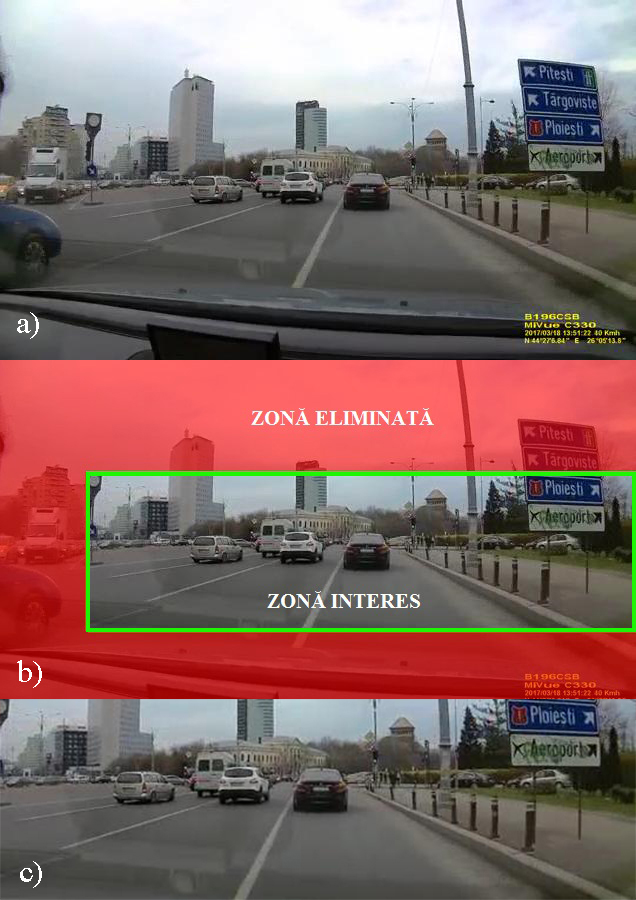
\includegraphics[max width=15cm,max height=15cm,keepaspectratio]{img_3_1}
	\caption[Zonă interes imagine]{a) Imaginea inițială b) Separația zonei de interes față de cea redundantă c) Imaginea de interes rezultată.}
\end{figure}

\subsubsection{Etapa 2: Obținere imagine IPM}

Următoare etapă în procesul de detecție a benzii curente de circulație este cea în care vom schimba perspectiva de vizualizare a zonei de interes. Prin intermediul unui fișier de configurare se vor da parametri ce vor fi folosiți ulterior în funcțiea de obținere IPM. Fie A, B, C și D punctele extreme ale imaginii. Vom redefini punctele B și C conform figurii 3.2. Cei doi vectori de puncte îi pasăm funcției $cv.getPerspectiveTransform$ din biblioteca OpenCV spre a obține matrice $M$ de trecere din perspectiva a), conform figurii 3.2, în perspectiva b). Matricea $M$ este folosită în continuare cu funcția $cv.warpPerspective$ pentru pentru a obține imaginea în planul IPM.
\begin{figure}[!h]
	\centering
	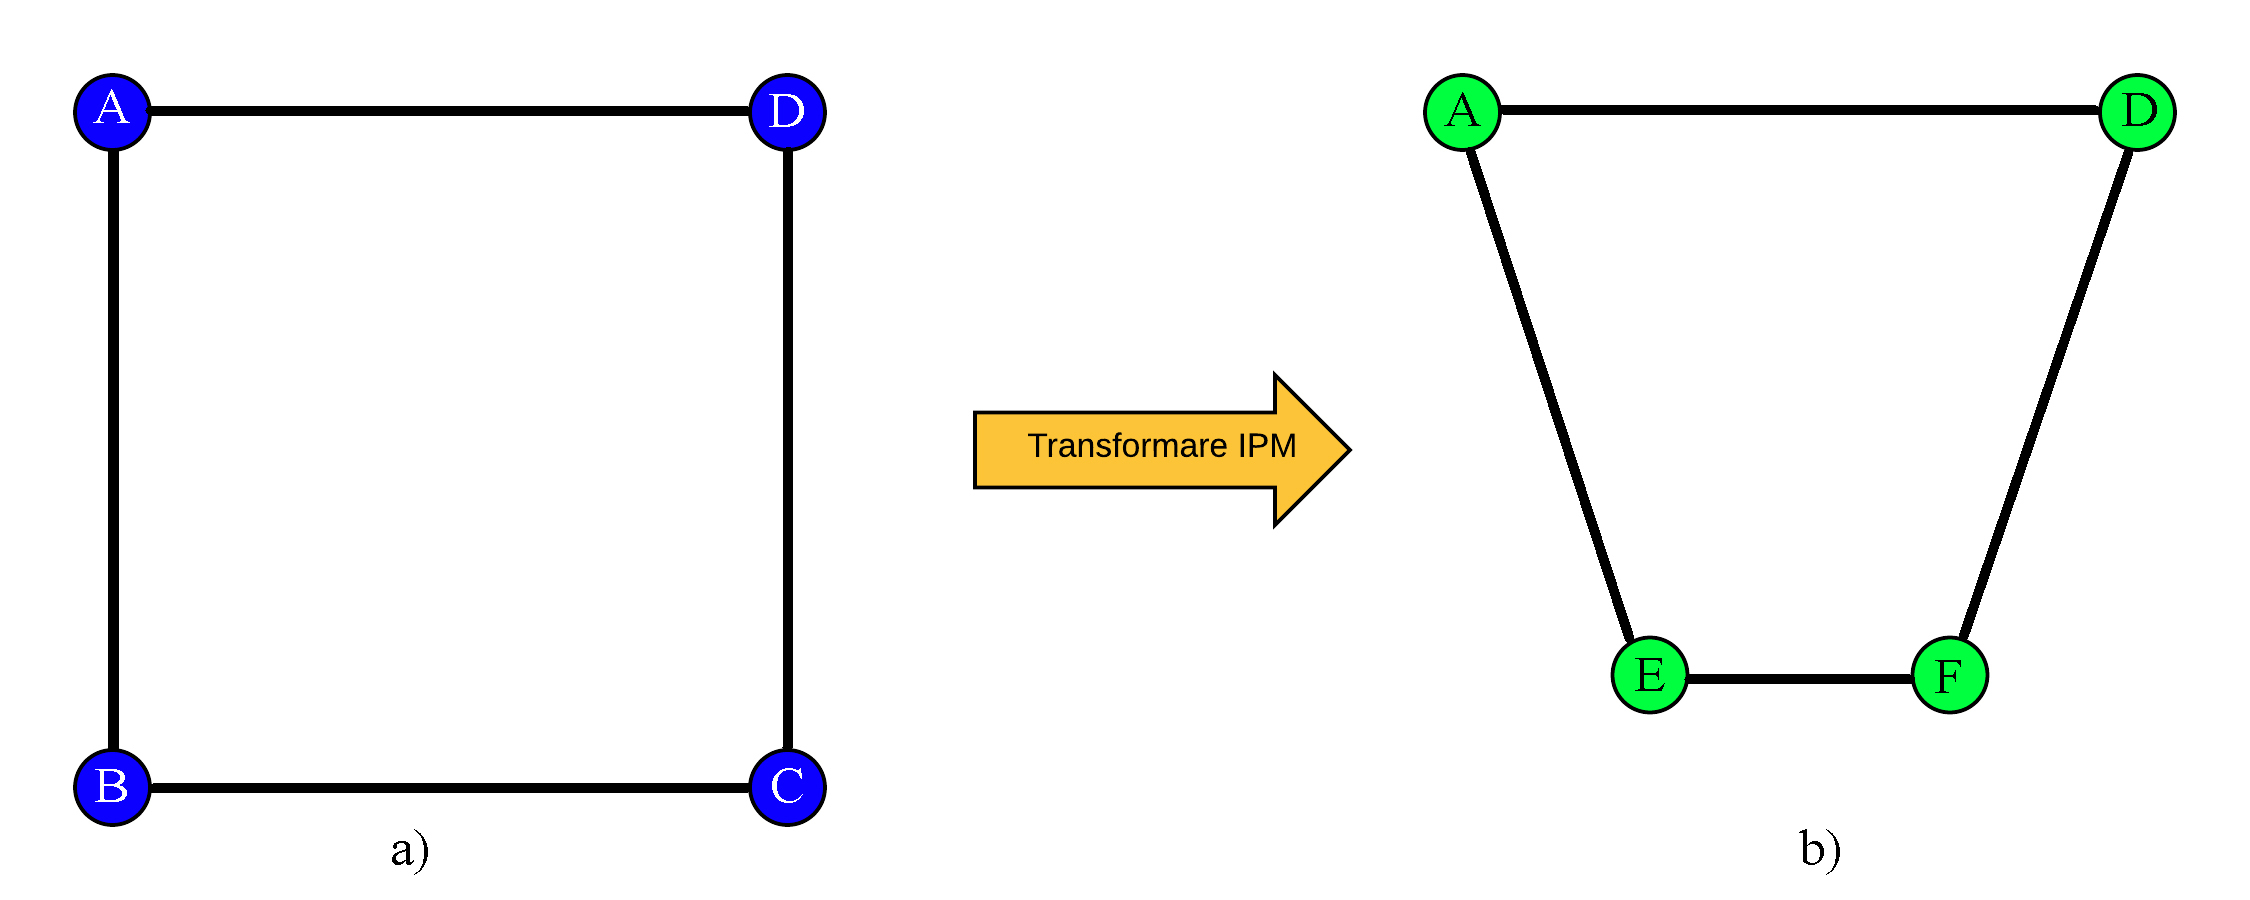
\includegraphics[max width=15cm,max height=15cm,keepaspectratio]{img_3_2}
	\caption[Transformare IPM]{a) Cadrul imaginii inițiale b) Cadrul imaginii IPM. Punctele B și C, din cadrul imaginii inițiale, sunt redefinite în punctele E și F.}
\end{figure}

În figura 3.3 este prezentat un exemplu practic.
\begin{figure}[!h]
	\centering
	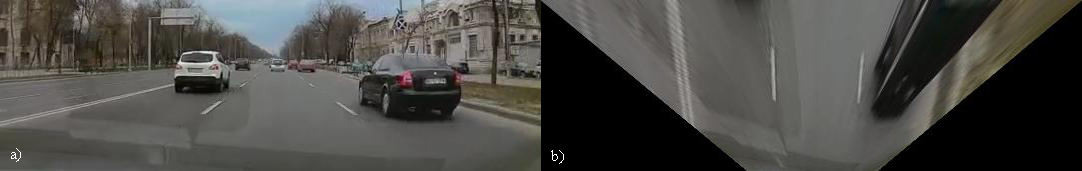
\includegraphics[max width=15cm,max height=15cm,keepaspectratio]{img_3_3}
	\caption[Transformare IPM în practică]{a) Imagine zonă interes b) Imaginea IPM asociată zonei de interes.}
\end{figure}


\subsubsection{Etapa 3: Filtrarea imaginii IPM}

Filtrarea imaginii IPM are rolul de a păstra în imagine doar zonele cele mai plauzibile de a fi marcaje delimitatorii de bandă și eliminarea celulalt conținut. Noua imagine, imagine, va fi o imagine binară de alb și negru. Pentru filtrare se folosește filtrul Gaussian orizontal
$ FG = 
\begin{bmatrix}
	0 & 0 & 0 \\
	0 & 1 & -1 \\
	0 & 0 & 0 \\
\end{bmatrix}
$
\begin{figure}[!h]
	\centering
	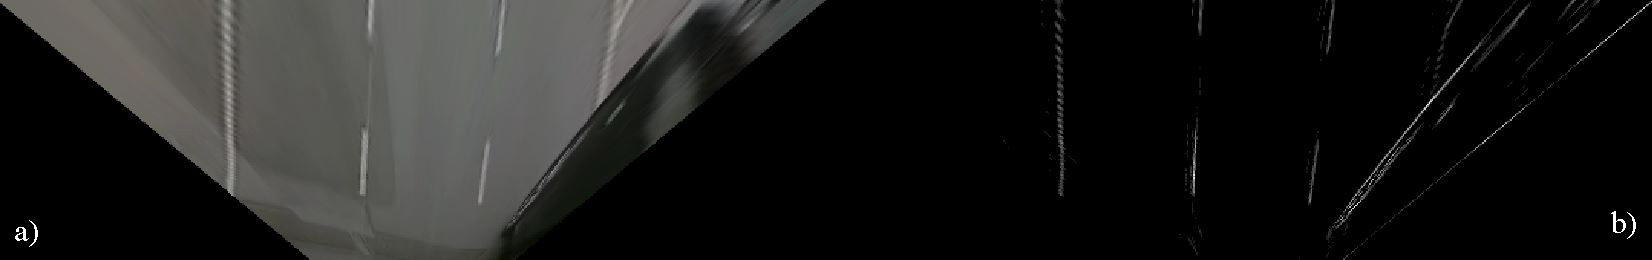
\includegraphics[max width=15cm,max height=15cm,keepaspectratio]{img_3_4}
	\caption[Imagine IPM filtrată]{a) Imaginea IPM b) Imaginea IPM filtrată.}
\end{figure}

\section{Detectare mașină}
\subsection{Noțiuni introductive}
\subsection{Algoritm detecție mașină}

\section{Determinare distanță}
\subsection{Noțiuni introductive}
\subsection{Algoritm determinare distanță}

\section{Determinare viteză relativă}
\subsection{Noțiuni introductive}
\subsection{Algoritm determinare viteză relativă}

\chapter{Baze de date}
\section{Bază de date benzi circulație}
\subsection*{Informații generale}

Partea din aplicație ce are rolul de a detecta banda curentă de circulație a fost dezvoltat plecând de la baza de date Caltech Lanes Dataset de imagini.  \hyperlink{Bazadedatebenzidecirculatie}{[4]}

\subsection*{Tipuri de imagini}

Caltech Lanes Dataset conține $1225$ de imagini cu adnotările de rigoare. Baza de date este împărțită în patru tipuri de clipuri și anume: $cordova1$ cu un număr total de 250 de imagini, $cordova2$ cu un număr total de 406 de imagini, $washington1$ cu un număr total de 337 de imagini și $washington2$ cu un număr total de 232 de imagini. Dintre aceste patru seturi de imagini au fost folosite cordova1, washington1 și washington2.

\begin{figure}[!h]
	\centering
	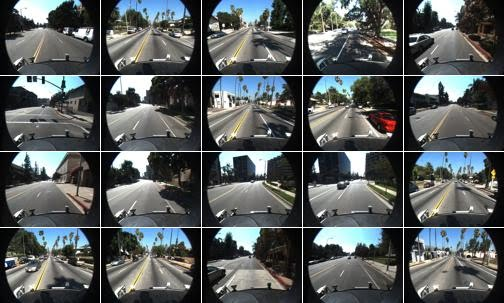
\includegraphics[max width=15cm,max height=15cm,keepaspectratio]{img_4_1}
	\caption[Imagini Caltech Lanes Dataset]{Exemple imagini din baza de date Caltech Lanes Dataset.}
\end{figure} 

\subsection*{Algoritm de evaluare}

Pentru evaluarea rezultatelor a fost folosit soft-ul de evaluare propus de autorul articolului Real time Detection of Lane Markers in Urban Streets \hyperlink{MohamedAly}{[11]}. 
Asupra acestuia au fost aduse modificări în privința citirii etichetelor asociate fiecărui video. Astfel, în cazul lucrării de față, accentul se pune pe banda curentă de circulație. Pentru a extrage doar aceste etichete au fost selectate conform distanței acestora față de centrul imaginii cu o încadrare într-un interval definit în prealabil.

\subsection*{Rezultate}

Aplicația are o precizie în detecție a benzilor de circulație pe video-urile analizate de $92.3\%$ detecții corecte și o rată de detecții false de $8.75\%$. Rezultatele detalitate pot fi vizualizate în tabelul 4.1.

\begin{table}[h!]
	\centering
	\begin{tabular}{||c | c | c | c | c | c ||} 
		\hline
		Video & Total frame-uri & Total linii & Detectații & Detecții corecte & Detecții false \\ [0.5ex] 
		\hline\hline
		cordova1 & 250 & 449 & 467 & 91.31\% & 12.69\%  \\ 
		washington1 & 336 & 667 & 662 & 88.48\% & 9.31\% \\
		washington2 & 232 & 448 & 454 & 97.10\% & 4.24\%  \\ 
		\hline\hline
		Total & 818 & 1 564 & 1 583 & 92.30\% & 8.75\% \\ [1ex]
		 
		\hline
	\end{tabular}
	\caption{Rezultate evaluare detecție bandă}
	\label{table:1}
\end{table}

În continuare pot fi vizualizate diverse exemple reușite, în figura 4.2, iar altele mai puțin reușite, în figura 4.3.

\begin{figure}[!h]
	\centering
	\includegraphics[max width=15cm,max height=15cm,keepaspectratio]{img_4_2}
	\caption[Detecție bandă - exemple reușite]{Exemple reușite. Rând 1 - cordova1, 2 - washington1, 3 - washington2.}
\end{figure}
\begin{figure}[!h]
	\centering
	\includegraphics[max width=15cm,max height=15cm,keepaspectratio]{img_4_3}
	\caption[Detecție bandă - exemple nereușite]{Exemple nereușite. Rând 1 - cordova1, 2 - washington1, 3 - washington2.}
\end{figure}

\section{Bază de date mașini}

\subsection*{Informații generale}

În cazul componentei ce se ocupă de detectarea mașinii au fost folosite două baze de date. Prima dintre aceasta, cea oferită de Universitatea Politehnică din Madrid și a fost folosită pentru antrenarea clasificatorilor \hyperlink{BazadedatemasiniUniversitateaPolitehnicadinMadrid}{[3]}.

Pentru testarea a fost folosită o altă bază de date cu imagini, oferită de Universitatea Oxford ce vine în completarea bazei de date oferite de Institutul de Tehnologie din California \hyperlink{BazadedatemasiniUniversitateaOxford}{[2}, \hyperlink{BazadedatemasiniInstituluideTehnologiedinCalifornia}{5]}.

\subsection*{Tipuri de imagini}

Baza de date oferită de Universitatea Politehnică din Madrid cuprinde două tipuri principale de imagini. Prima categorie conține imagini cu mașini și este împărțită în alte patru subcategori: mașini fotografiate din stânga, mașini fotografiate din dreapta, mașini fotografiate din depărtare și mașini fotografiate din centru. Aceste patru subcategori însumează un număr total de 3 425 de imagini. Aceste imagini provin din diferite condiții, spre exemplu imagini din vreme însorită, înorată, condiții medii, ploaie, iluminat artificial sau iluminare slabă.

A doua parte a acestei baze de date este reprezentată de imaginile de antrenare negative, ce nu conțin mașini. La rândul lor sunt împărțite în cele patru subcategori menționate anterior și însumează un număr total de 3 900 de imagini.

Baza oferită de Universitatea Oxford este formată la rândul ei din alte două baze de date de imagini. Aceste imagini nu au venit insoțite de etichete, astfel etichetarea a fost făcută ulterior. Din contopirea celor 2 baze de date a rezultat un set de 987 de imagini cu mașini pentru testare.

\subsection*{Algoritm de evaluare}

În ceea ce privește algoritmul de evaluare, fiecare fereastră ce poate conține o mașină oferită de aplicație a fost comparată cu etichetele asociate imaginii respective, iar dacă suprapunere dintre locația indicată de aplicație și locația etichetată se află într-un anumit prag predefinit este acceptată ca detecție adevărată, în caz contrar, este clasificată ca fiind o detecție falsă.

\subsection*{Rezultate}

Precizia medie obțiuntă de aplicație este de 91.30\% după cum se poate observa în figura 4.4.

\begin{figure}[!h]
	\centering
	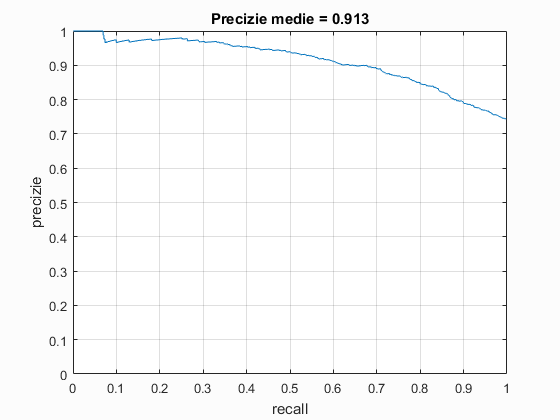
\includegraphics[max width=15cm,max height=15cm,keepaspectratio]{img_4_4}
	\caption{Grafic precizie - recall detecție mașină}
\end{figure}

În figura 4.5 și 4.6 sunt prezentate exemple reușite și exemple nereușite. 

\begin{figure}[!h]
	\centering
	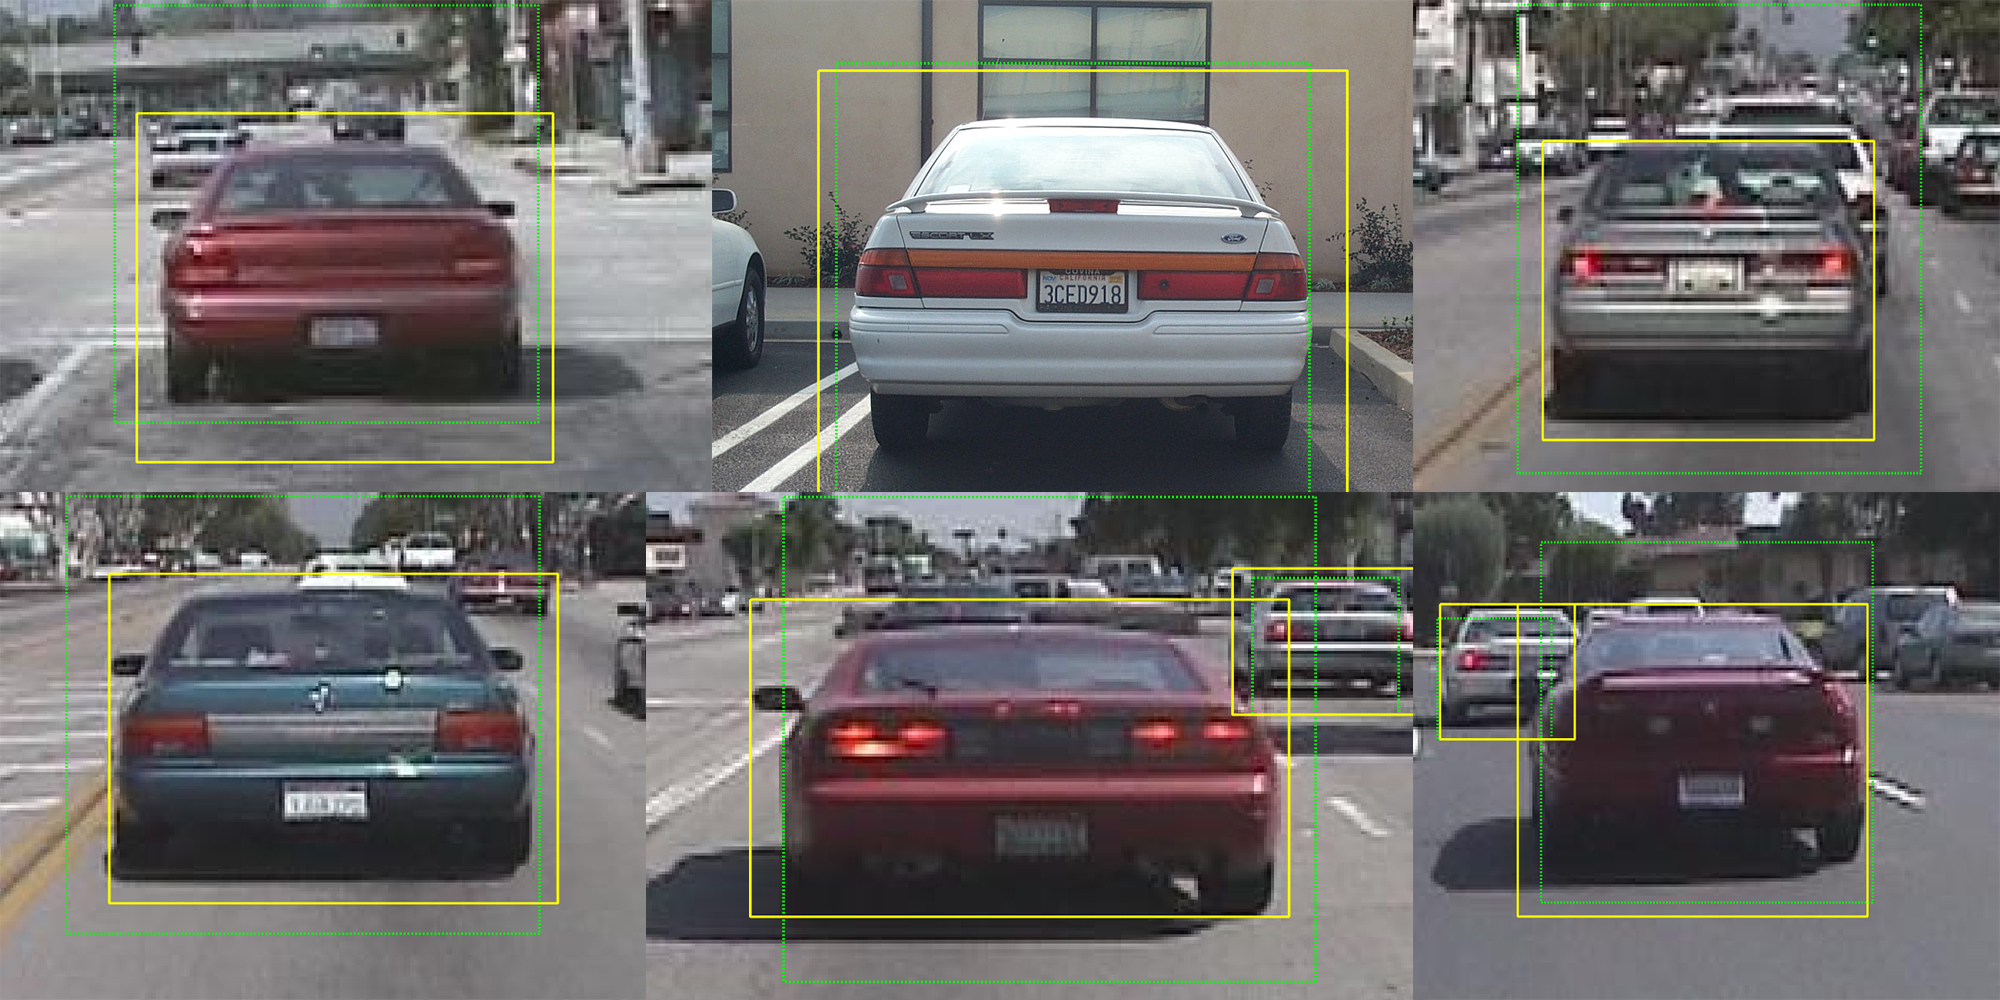
\includegraphics[max width=15cm,max height=15cm,keepaspectratio]{img_4_5}
	\caption{Detecție mașini - exemple reușite}
\end{figure}
\begin{figure}[!ht]
	\centering
	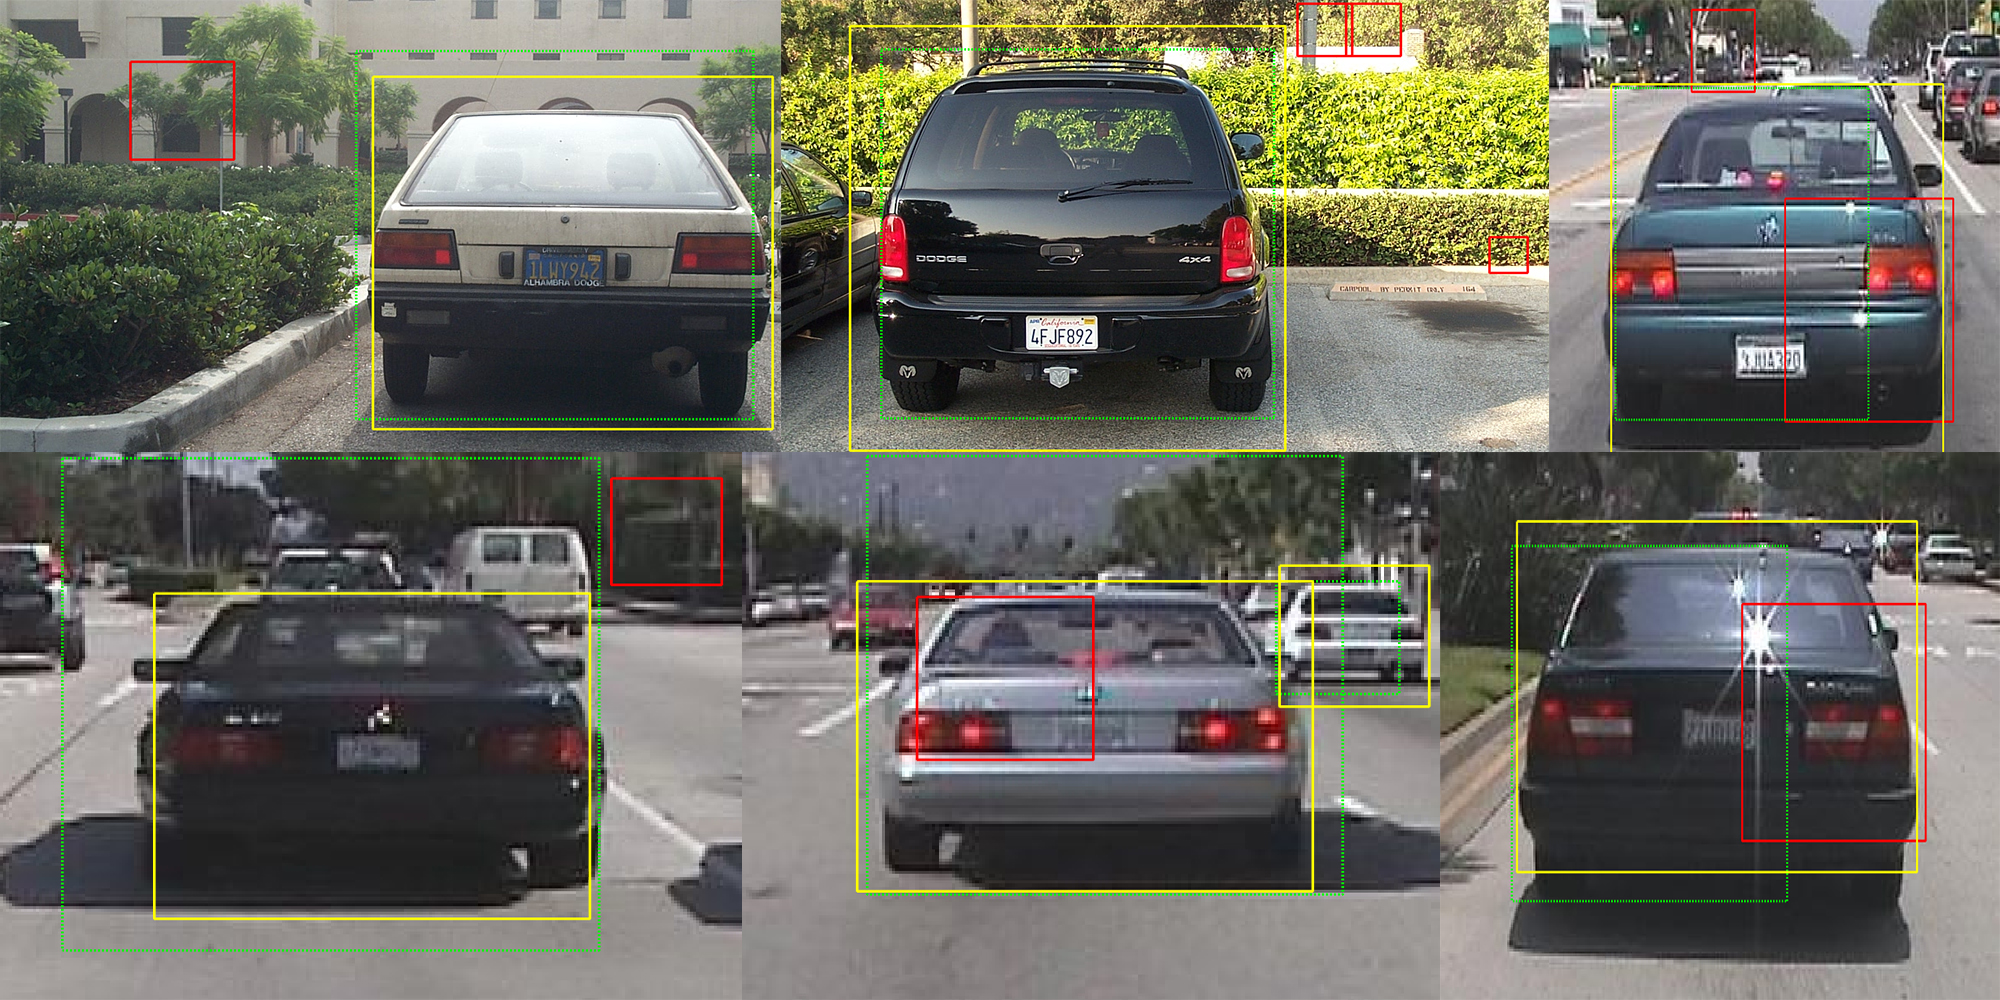
\includegraphics[max width=15cm,max height=15cm,keepaspectratio]{img_4_6}
	\caption{Detecție mașini - exemple nereușite}
\end{figure}

\newpage\null\newpage
\chapter*{Concluzii}
\section*{Concluzii generale}
Prezenta lucrare a abordat cu succes cele patru componente dezvoltate. Precizia de detecție a fost atât în cazul detectării de bandă de circulație, însă doar în situațiile în care marcajele rutiere tind în general să fie drepte, cât și în cazul detectării mașinii aflate pe respectiva bandă, de peste 90\%. Aceste rezultate confirmă abordarea finalizată cu succes a aplicației.  

În ceea ce privește determinarea distanței și a vitezei relative putem afirma că este un început acceptabil, însă necesită o dezvoltare mai concretă într-o versiune ulterioară.

Din punct de vedere practic, aplicația poate fi folosită cu rol consultativ. O versiune ulterioară a acesteia cu mențiunile specificate în continuare poate fi chiar conectată la sistemul mașinii.

\section*{Direcții viitoare de dezvoltare}
Dintre posibilele direcții vitoare de dezvoltare a aplicației curente, putem menționa următoarele.

\textbf{Diferențiere marcaj linie}

Într-o versiune ulterioară a acestei aplicații se poate implementa un sistem ce are capacitatea de a face diferența dintre liniile discontinue și cele continue, iar în situația în care conducătorul mașinii depășește linia continuă să fie avertizat cu privire la acest aspect.

\textbf{Determinare viteză de deplasare}

O altă posibilă caracteristică adusă prezentei aplicații este reprezentată de determinarea vitezei de deplasare. Astfel pe lângă determinarea vitezei relative ce ne specifică cu cât mai repede sau cu cât mai încet se deplasază mașina din față, să poate specifica și care este viteza curentă de deplasare a mașinii din care este inregistrat video-ul.

\textbf{Detectare indicatoare rutiere}

De asemenea, detectarea indicatoarelor rutiere este o componentă esențială într-o versiune ulterioare a aplicației curente. Aceasta prespune identificarea tuturor tipurilor de indicatoarelor rutiere și oferirea de avertizmente în funcție de indicatorul rutier detectat și de semnificația acestuia.

\textbf{Detectarea liniilor curbate}

În această variantă preliminară, aplicația are capacitatea de a detecta doar liniile drepte asociate benzii de circulație. Însă, în multe situații se întamplă ca aceste linii să se afle într-o curbă, ceea ce face ca actuala componentă de detectare a benzii de circulație să nu funcționeze la fel de bine. Fapt ce poate fi observat în figura 5.1.

\renewcommand{\thefigure}{5.\arabic{figure}}
\setcounter{figure}{0}
\begin{figure}[!h]
	\centering
	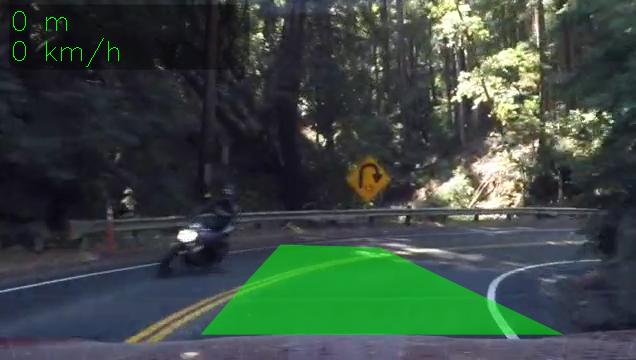
\includegraphics[max width=15cm,max height=15cm,keepaspectratio]{img_5_1}
	\caption{Detecție linii curbe}
\end{figure} 

\begin{thebibliography}{9}
	
	\bibitem{AnuarMikdadMuadAiniHussainSalinaAbdulSamadMohdMarzukiMustaffaBurhanuddinYeopMajlis}
	\hypertarget{AnuarMikdadMuadAiniHussainSalinaAbdulSamadMohdMarzukiMustaffaBurhanuddinYeopMajlis}{} 
	Anuar Mikdad Muad, Aini Hussain, Salina Abdul Samad, Mohd. Marzuki Mustaffa, Burhanuddin Yeop Majlis.
	\textit{\href{http://ieeexplore.ieee.org/abstract/document/1414393/}{Implementation of inverse perspective mapping algorithm for the development of an automatic lane tracking system}}.
	TENCON 2004. 2004 IEEE Region 10 Conference, 207 - 210, 2004.
		
	\bibitem{BazădedateautovehicoleUniversitateaOxford}
	\hypertarget{BazădedateautovehicoleUniversitateaOxford}{} 
	Bază de date autovehicole Universitatea Oxford
	\\\texttt{\url{http://www.robots.ox.ac.uk/~vgg/data3.html}}
	
	\bibitem{BazădedateautovehicoleUniversitateaPolitehnicădinMadrid}
	\hypertarget{BazădedateautovehicoleUniversitateaPolitehnicădinMadrid}{} 
	Bază de date autovehicole Universitatea Politehnică din Madrid
	\\\texttt{\url{http://www.gti.ssr.upm.es/data/Vehicle\_database.html}}
	
	\bibitem{Bazădedatebenzidecirculație}
	\hypertarget{Bazădedatebenzidecirculație}{} 
	Bază de date benzi de circulație
	\\\texttt{\url{http://www.mohamedaly.info/datasets/caltech-lanes}}
	
	\bibitem{BazădedatemașiniInstituluideTehnologiedinCalifornia}
	\hypertarget{BazădedatemașiniInstituluideTehnologiedinCalifornia}{} 
	Bază de date mașini Institului de Tehnologie din California
	\\\texttt{\url{http://www.vision.caltech.edu/html-files/archive.html}}
	
	\bibitem{ChristopherBishop}
	\hypertarget{ChristopherBishop}{} 
	Christopher M. Bishop. 
	\textit{Pattern Recognition and Machine Learning}. 
	Springer, New York, 2006.
	
	\bibitem{CorinnaCortesVladimirVapnik}
	\hypertarget{CorinnaCortesVladimirVapnik}{} 
	Corinna Cortes and Vladimir Vapnik.
	\textit{\href{http://image.diku.dk/imagecanon/material/cortes_vapnik95.pdf}{Support-Vector Networks}}.
	Machine Learning, 20, 273 - 297:1 - 25, 1995.
	
	\bibitem{Dinamicaaccidentelorrutiere}
	\hypertarget{Dinamicaaccidentelorrutiere}{}  
	Dinamica accidentelor rutiere
	\\\texttt{\url{https://www.politiaromana.ro/ro/structura-politiei-romane/unitati-centrale/directia-rutiera/statistici}}
		
	\bibitem{ErinAllweinRobertSchapireYoramSinger}
	\hypertarget{ErinAllweinRobertSchapireYoramSinger}{} 
	Erin Allwein, Robert Schapire and Yoram Singer.
	\textit{\href{http://www.jmlr.org/papers/volume1/allwein00a/allwein00a.pdf}{Reducing multiclass to binary: a unifying approach for margin classifiers}}.
	Journal of Machine Learning Research 1, 113 – 141, 2000.
	
	\bibitem{JasonWestonSimonWatkins}
	\hypertarget{JasonWestonSimonWatkins}{} 
	Jason Weston and Simon Watkins.
	\textit{\href{https://www.elen.ucl.ac.be/Proceedings/esann/esannpdf/es1999-461.pdf}{Support Vector Machines for Multi-Class Pattern Recognition}}.
	ESANN, 1 - 6, 1995.
	
	\bibitem{MohamedAly}
	\hypertarget{MohamedAly}{}  
	Mohamed Aly.
	\textit{\href{http://www.vision.caltech.edu/malaa/publications/aly08realtime.pdf}{Real time Detection of Lane Markers in Urban Streets}}.
	1 - 6, 2008.
	
	\bibitem{NavneetDalalBillTriggs}
	\hypertarget{NavneetDalalBillTriggs}{}  
	Navneet Dalal and Bill Triggs. 
	\textit{\href{https://hal.inria.fr/file/index/docid/548512/filename/hog\_cvpr2005.pdf}{Histograms of Oriented Gradients for Human Detection}}.
	1 - 9, 2005.
		
	\bibitem{RichardSzeliski}
	\hypertarget{RichardSzeliski}{}
	Richard Szeliski. 
	\textit{Computer Vision: Algorithms and Applications}. 
	Springer, London, 2010.
		
	\bibitem{ShaneTuohyEdwardJonesMartinGlavin}
	\hypertarget{ShaneTuohyEdwardJonesMartinGlavin}{} 
	Shane Tuohy, Edward Jones and Martin Glavin
	\textit{\href{https://www.researchgate.net/profile/Martin\_Glavin/publication/224195999\_Distance\_determination\_for\_an\_automobile\_environment\_using\_Inverse\_Perspective\_Mapping\_in\_OpenCV/links/00b4951c994745bf6b000000/Distance-determination-for-an-automobile-environment-using-Inverse-Perspective-Mapping-in-OpenCV.pdf}{Distance determination for an automobile environment using Inverse Perspective Mapping in OpenCV}}.
	1 - 6, 2010.
		
	\bibitem{SoviraTanJasonDaleAndrewAndersonAlanJohnston}
	\hypertarget{SoviraTanJasonDaleAndrewAndersonAlanJohnston}{} 
	Sovira Tan, Jason Dale, Andrew Anderson and Alan Johnston.
	\textit{\href{https://www.researchgate.net/profile/Alan\_Johnston2/publication/222433205\_Inverse\_Perspective\_Mapping\_and\_Optic\_Flow\_A\_Calibration\_Method\_and\_a\_Quantitative\_Analysis/links/53f4986c0cf22be01c3ed295/Inverse-Perspective-Mapping-and-Optic-Flow-A-Calibration-Method-and-a-Quantitative-Analysis.pdf}{Inverse perspective mapping and optic flow: A calibration method and a quantitative analysis}}.
	1 - 13, 2005.
		
	\bibitem{TeslaAutopilotSystem}
	\hypertarget{TeslaAutopilotSystem}{} 
	Tesla Autopilot System
	\\\texttt{\url{https://www.tesla.com/en\_GB/autopilot}}
		
	\bibitem{TheAtlantic}
	\hypertarget{TheAtlantic}{} 
	Self-Driving Cars Could Save 300,000 Lives Per Decade in America
	\\\texttt{\url{https://www.theatlantic.com/technology/archive/2015/09/self-driving-cars-could-save-300000-lives-per-decade-in-america/407956/?utm\_source=SFTwitter}}
		
	\bibitem{ThomasDietterichGhulumBakiri}
	\hypertarget{ThomasDietterichGhulumBakiri}{} 
	Thomas Dietterich and Ghulum Bakiri.
	\textit{\href{http://www.jair.org/media/105/live-105-1426-jair.pdf}{Solving Multiclass Learning Problems via Error-Correcting Output Codes}}.
	Journal of Artificial Intelligence Research 2, 263 – 286:1 - 24, 1995.
		
	\bibitem{VladimirVapnik}
	\hypertarget{VladimirVapnik}{}  
	Vladimir Vapnik. 
	\textit{Statistical Learning Theory}. 
	Wiley, New York, 1998.
		
	\bibitem{WaymoSystem}
	\hypertarget{WaymoSystem}{} 
	Waymo System
	\\\texttt{\url{https://waymo.com/}}

\end{thebibliography}

\end{document}